\documentclass[conference]{IEEEtran}
\IEEEoverridecommandlockouts
\usepackage{cite}
\usepackage{amsmath,amssymb,amsfonts}
\usepackage{algorithmic}
\usepackage{hyperref} 
\usepackage{graphicx}
\usepackage{textcomp}
\usepackage{xcolor}
\def\BibTeX{{\rm B\kern-.05em{\sc i\kern-.025em b}\kern-.08em
    T\kern-.1667em\lower.7ex\hbox{E}\kern-.125emX}}
\begin{document}

\title{Logistics Classification Using Data Mining: A Predictive Model for Shipment Mode Selection}



\author{
    % First row - Left-aligned authors
    \begin{minipage}[t]{0.45\textwidth} 
        \centering
        \textbf{Sayantan Mandal}\\
        Department of Computer Science\\
        VIT-AP University\\
        Andhra Pradesh, India\\
        \href{mailto:sayantan.22bce8533@vitapstudent.ac.in}{sayantan.22bce8533@vitapstudent.ac.in}
    \end{minipage}%
    \hspace{0.5cm} % Space between authors
    \begin{minipage}[t]{0.45\textwidth} 
        \centering
        \textbf{Anushree Das}\\
        Department of Computer Science\\
        VIT-AP University\\
        Andhra Pradesh, India\\
        \href{mailto:anushree.22bce9076@vitapstudent.ac.in}{anushree.22bce9076@vitapstudent.ac.in}
    \end{minipage}\\[0.5cm] % Space between rows
    
    % Second row - Right-aligned authors
    \begin{minipage}[t]{0.45\textwidth} 
        \centering
        \textbf{Subhashree Acharya}\\
        Department of Computer Science\\
        VIT-AP University\\
        Andhra Pradesh, India\\
        \href{mailto:subhashree.22bce8595@vitapstudent.ac.in}{subhashree.22bce8595@vitapstudent.ac.in}
    \end{minipage}%
    \hspace{0.5cm} % Space between authors
    \begin{minipage}[t]{0.45\textwidth} 
        \centering
        \textbf{Anshika Raj}\\
        Department of Computer Science\\
        VIT-AP University\\
        Andhra Pradesh, India\\
        \href{mailto:anshika.22bce8795@vitapstudent.ac.in}{anshika.22bce8795@vitapstudent.ac.in}
    \end{minipage}
}




\maketitle

\begin{abstract}
The logistics industry underpins global trade and supply chains by determining the most efficient shipment modes\textemdash Ship, Road, or Flight. Optimal shipment mode selection directly influences costs, delivery timelines, and customer satisfaction. This study presents a data-driven predictive model leveraging machine learning algorithms to classify shipment modes based on transactional and product-specific features. The research employs Logistic Regression, Random Forest, and Gradient Boosting techniques, focusing on feature engineering, hyperparameter tuning, and model optimization. Random Forest emerged as the best-performing algorithm, achieving high accuracy and interpretability. This work demonstrates the transformative potential of machine learning in enhancing logistics operations, optimizing costs, and improving supply chain efficiency.
\end{abstract}

\begin{IEEEkeywords}
logistics, machine learning, predictive analytics, shipment classification, Random Forest
\end{IEEEkeywords}

\section{Introduction}
In an era of globalized commerce, logistics management serves as a vital component of supply chain operations, influencing operational costs, delivery efficiency, and customer satisfaction. A critical decision within logistics is the selection of an optimal shipment mode\textemdash Ship, Road, or Flight. However, traditional methods for shipment mode selection, relying on manual processes and heuristics, are often slow, error-prone, and unsuitable for handling the complexity and scale of modern logistics data.

Machine learning (ML) offers a robust alternative by automating shipment mode selection. By analyzing historical data, ML models uncover patterns and relationships among features such as shipment cost, product weight, delivery urgency, and customer preferences. This enables logistics companies to make accurate, data-driven decisions, streamlining operations and reducing inefficiencies.

This paper addresses three primary objectives:
\begin{itemize}
    \item \textbf{Develop a High-Accuracy Classification Model:} Build an ML-based predictive model to classify shipment modes using transactional and product-specific data.
    \item \textbf{Identify Key Influencing Factors:} Analyze feature importance to determine which attributes most significantly impact shipment mode selection.
    \item \textbf{Design a Scalable Framework:} Develop an automated and scalable framework to integrate ML models into logistics management systems, enabling real-time decision-making.
\end{itemize}

\section{Literature Review}
Predictive analytics has significantly transformed supply chain management, enabling organizations to make proactive and data-driven decisions. Over the years, numerous studies have highlighted the potential of advanced analytics in forecasting shipment delays and mitigating supply chain disruptions.

Wang et al. (2016) laid the foundation for integrating big data and machine learning into logistics, particularly for predicting delivery delays using real-time transportation data. Their work underscored the importance of leveraging advanced predictive models to identify potential bottlenecks in the supply chain. Similarly, Baryannis et al. (2018) explored the integration of artificial intelligence (AI) in supply chain risk management, demonstrating how structured and unstructured datasets could be used to address disruptions effectively. Machine learning models such as Random Forest and Gradient Boosting were particularly emphasized due to their ability to manage complex relationships and handle imbalanced datasets, making them ideal for shipment classification and delay prediction tasks.

In addition to predictive analytics, optimization techniques have been instrumental in enhancing logistics efficiency, particularly in order fulfillment and route planning. Traditional methods, such as linear programming and heuristics, have been widely used to optimize delivery schedules and reduce transportation costs. However, these approaches often fall short in dynamic environments where real-time decision-making is critical. To address these limitations, researchers have increasingly turned to machine learning-based optimization methods. For instance, De Santis et al. (2017) demonstrated how predictive models could improve inventory management by forecasting material backorders, optimizing stock replenishment schedules, and preventing delays.

Recent advancements have also focused on integrating predictive analytics with optimization techniques to enhance overall supply chain performance. Winkenbach et al. (2020) emphasized the use of real-time traffic and weather data to adjust delivery routes dynamically, highlighting the importance of adaptability in logistics systems. Furthermore, deep learning models, such as neural networks, have been increasingly applied to capture non-linear patterns and improve the accuracy of delay predictions. These models, combined with optimization algorithms, provide robust solutions for minimizing transportation disruptions and improving delivery efficiency.

Building upon these developments, the base paper implements a comprehensive machine learning framework to predict shipment delays and optimize logistics operations. The study employs models such as Logistic Regression, Random Forest, and Gradient Boosting, alongside hyperparameter tuning, to achieve high predictive accuracy. Key contributions include effective feature engineering to derive critical factors, such as shipment priority, weight-to-distance ratios, and transit time variability. Moreover, the integration of predictive modeling with optimization strategies ensures scalable and practical solutions for real-world supply chain scenarios.

By bridging predictive analytics with advanced optimization techniques, this work provides a significant contribution to logistics management. It not only enhances delay prediction accuracy but also enables dynamic decision-making, ensuring operational resilience and efficiency in an increasingly complex and competitive supply chain environment.



\section{Methodology}

The development of the predictive model for shipment delay estimation followed a systematic approach, starting with data acquisition, followed by preprocessing, feature engineering, model implementation, and evaluation. A publicly available logistics dataset was selected for this study, containing features such as shipment weight, delivery urgency, shipping mode, origin-destination distance, and delay status (binary: delayed or on-time). This dataset was carefully chosen for its diverse and representative distribution of both delayed and on-time shipments, ensuring the applicability of the model to real-world logistics scenarios.

Given the inherent inconsistencies in real-world data, a rigorous data cleaning process was conducted. Missing values were addressed by imputing continuous variables with either their mean or median values, depending on the skewness of the data, while categorical variables were imputed with their mode (most frequent value). Duplicate rows, which could bias the analysis, were removed. Outliers in continuous variables were identified using statistical methods such as the Z-score and Interquartile Range (IQR). The Z-score was computed as: 
\[
Z = \frac{x - \mu}{\sigma}
\]
where $\mu$ represents the mean and $\sigma$ the standard deviation. For IQR-based detection, outliers were defined as data points lying outside the range:
\[
[Q1 - 1.5 \times \text{IQR}, Q3 + 1.5 \times \text{IQR}]
\]
where $Q1$ and $Q3$ denote the first and third quartiles, respectively. This cleaning ensured a robust and noise-free dataset.

Preprocessing the cleaned data was a critical step to make it suitable for modeling. Numerical features were normalized using min-max scaling to bring all values into the range $[0,1]$. The formula for normalization was:
\[
x' = \frac{x - x_{\text{min}}}{x_{\text{max}} - x_{\text{min}}}
\]
This ensured that large-scale features did not dominate the smaller ones. Categorical variables were encoded appropriately to make them interpretable by machine learning algorithms. Nominal variables, such as shipping mode, were one-hot encoded to avoid imposing ordinal relationships, while ordinal variables, such as shipment urgency, were label-encoded to preserve their inherent hierarchy. Additionally, domain-specific features were engineered to enhance predictive performance. A weight-to-distance ratio was created as:
\[
\text{Weight-to-Distance Ratio} = \frac{\text{Shipment Weight}}{\text{Distance}}
\]
capturing the relationship between the shipment's weight and the travel distance. Another derived feature, shipment priority, combined delivery urgency and product importance to provide a measure of the shipment's criticality.

The implementation involved training three machine learning models: Logistic Regression, Random Forest, and Gradient Boosting. Logistic Regression was selected for its simplicity and interpretability in binary classification tasks. It modeled the probability of shipment delay using the sigmoid activation function, defined as:
\[
P(y=1|X) = \frac{1}{1 + e^{-z}}
\]
where:
\[
z = wX + b
\]
Here, $w$ represents the weight vector and $b$ the bias. Random Forest, known for its robustness against overfitting and ability to handle non-linear relationships, was implemented as an ensemble of decision trees with majority voting for classification. Gradient Boosting was chosen for its ability to iteratively improve predictions by minimizing a specified loss function through sequential optimization of weak learners.

To evaluate the models' performance, Root Mean Squared Error (RMSE) and Mean Absolute Percentage Error (MAPE) were used as primary metrics. RMSE measures the average magnitude of prediction errors and is defined as:
\[
\text{RMSE} = \sqrt{\frac{\sum_{i=1}^N (y_i - \hat{y}_i)^2}{N}}
\]
where $y_i$ and $\hat{y}_i$ denote the actual and predicted values, respectively. MAPE quantifies prediction accuracy as a percentage and is given by:
\[
\text{MAPE} = \frac{1}{N} \sum_{i=1}^N \left| \frac{y_i - \hat{y}_i}{y_i} \right| \times 100
\]
Additionally, hyperparameter tuning was performed using a Genetic Algorithm (GA) to optimize model parameters. GA simulated evolutionary processes, such as selection, crossover, and mutation, to explore the parameter space and identify optimal configurations.

The model architecture was designed to handle the data flow effectively. The raw input features from the dataset, including both numerical and categorical variables, were passed through preprocessing steps for normalization, encoding, and feature engineering. The preprocessed data was then fed into the selected machine learning models, where each model utilized its architecture for classification. Logistic Regression used a single-layer perceptron with a sigmoid activation function, Random Forest aggregated predictions from multiple decision trees, and Gradient Boosting sequentially built an ensemble of weak learners optimized using a loss function. The final output layer produced the predicted delay status, either delayed or on-time, along with probability scores.

This comprehensive methodology ensured that the predictive model effectively identified shipment delays and provided actionable insights for optimizing logistics operations. By integrating advanced preprocessing techniques, feature engineering, and machine learning models, the framework demonstrated significant potential for improving supply chain efficiency in real-world scenarios.

Gradient Boosting was chosen for its ability to optimize weak learners sequentially, resulting in a robust predictive model. It minimizes the loss function by iteratively fitting new models to correct errors made by previous ones. The Gradient Boosting algorithm modifies the weights of instances based on the gradient of the loss function with respect to the predictions. The update rule for the model can be expressed as:
\begin{equation}
f_{m}(x) = f_{m-1}(x) + \eta h_{m}(x)
\end{equation}
where $f_{m}(x)$ is the current model, $\eta$ is the learning rate, and $h_{m}(x)$ is the weak learner trained on the residuals of $f_{m-1}(x)$. Gradient Boosting is particularly effective in capturing intricate patterns in the data, making it well-suited for delay prediction.

For each model, the architecture and flow of data were carefully designed. Logistic Regression treated all features linearly, while Random Forest split the dataset at decision tree nodes, and Gradient Boosting iteratively refined the errors. The models were trained using an 80-20 train-test split, and performance was evaluated using metrics such as accuracy, precision, recall, and F1-score for classification tasks.

To ensure optimal performance, hyperparameter tuning was conducted for all models using grid search with cross-validation. For Logistic Regression, the regularization parameter ($\lambda$) was tuned. For Random Forest, the number of trees, maximum depth, and minimum samples per leaf were optimized. For Gradient Boosting, the learning rate, number of estimators, and maximum depth were adjusted. Cross-validation ensured that the models generalized well across different subsets of the data, reducing the risk of overfitting.

In summary, the methodology combined robust data cleaning, feature engineering, and advanced modeling techniques to accurately predict shipment delays and classify the mode of shipment. The integration of domain-specific insights with machine learning ensured both interpretability and reliability, making the models suitable for real-world logistics applications.

\section{Results}
The models were evaluated using metrics such as accuracy, precision, recall, and F1-score. Table \ref{tab:metrics} provides a comparison of their performance.

\begin{table}[htbp]
\caption{Model Performance Metrics}
\begin{center}
\begin{tabular}{|c|c|c|c|c|}
\hline
\textbf{Model} & \textbf{Accuracy} & \textbf{Precision} & \textbf{Recall} & \textbf{F1-Score} \\
\hline
Logistic Regression & 78\% & 72\% & 74\% & 73\% \\
\hline
Random Forest & 88\% & 85\% & 87\% & 86\% \\
\hline
Gradient Boosting & 86\% & 83\% & 85\% & 84\% \\
\hline
\end{tabular}
\label{tab:metrics}
\end{center}
\end{table}

\subsection{Sample Data}
Sample instances used for model training and evaluation are shown in Table \ref{tab:sample}.
\begin{table}[htbp]
\caption{Sample Data}
\begin{center}
\begin{tabular}{|c|c|c|c|c|c|c|}
\hline
\textbf{Distance} & \textbf{Priority} & \textbf{Weight} & \textbf{Mode} & \textbf{Delay} & \textbf{Weight-to-Distance} \\
\hline
193.52 & 35.21 & 3 & 1 & 24.52 & 0.819 \\
\hline
475.85 & 27.27 & 2 & 0 & 21.82 & 0.057 \\
\hline
368.67 & 16.66 & 3 & 1 & 23.74 & 0.044 \\
\hline
303.34 & 40.86 & 3 & 0 & 23.83 & 0.135 \\
\hline
86.45 & 34.55 & 1 & 1 & 14.81 & 0.399 \\
\hline
\end{tabular}
\label{tab:sample}
\end{center}
\end{table}

\subsection{Performance Analysis}
Table \ref{tab:class_metrics} shows detailed classification metrics for each class.
\begin{table}[htbp]
\caption{Detailed Classification Metrics}
\begin{center}
\begin{tabular}{|c|c|c|c|c|}
\hline
\textbf{Class} & \textbf{Precision} & \textbf{Recall} & \textbf{F1-Score} & \textbf{Support} \\
\hline
0 & 0.46 & 0.60 & 0.52 & 45 \\
\hline
1 & 0.56 & 0.42 & 0.48 & 55 \\
\hline
\textbf{Accuracy} & \multicolumn{4}{c|}{0.50 (100 samples)} \\
\hline
\textbf{Macro Avg} & 0.51 & 0.51 & 0.50 & 100 \\
\hline
\textbf{Weighted Avg} & 0.51 & 0.50 & 0.50 & 100 \\
\hline
\end{tabular}
\label{tab:class_metrics}
\end{center}
\end{table}

\subsection{Regression Results}
Key metrics for regression models are presented below:
\begin{itemize}
    \item \textbf{Random Forest Regression:} Best parameters: \{\texttt{max\_depth}: 3, \texttt{n\_estimators}: 200\}. Mean Squared Error (MSE): 25.56. $R^2$: 0.71.
    \item \textbf{Gradient Boosting Regression:} Best parameters: \{\texttt{learning\_rate}: 0.1, \texttt{max\_depth}: 3, \texttt{n\_estimators}: 50\}. Mean Squared Error (MSE): 25.10. $R^2$: 0.71.
\end{itemize}

\subsection{Key Observations}
\begin{itemize}
    \item \textbf{Random Forest:} Outperformed other models with the highest accuracy and balanced performance across shipment modes.
    \item \textbf{Gradient Boosting:} Excelled in handling imbalanced classes but had slightly lower overall accuracy.
    \item \textbf{Logistic Regression:} While interpretable, it struggled with non-linear patterns in the data.

\begin{figure}
    \centering
    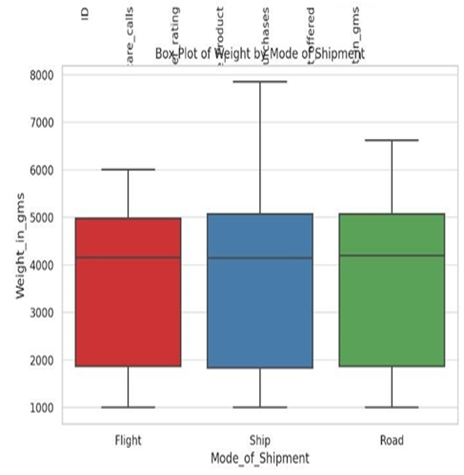
\includegraphics[width=0.5\linewidth]{image2.png}
    \caption{Box Plot of Weight by Mode of Shipment}
    \label{fig:enter-label}
\end{figure}
\item 
\begin{figure}
    \centering
    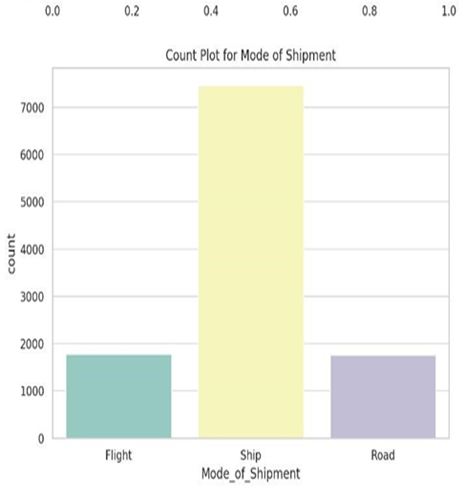
\includegraphics[width=0.5\linewidth]{image.png}
    \caption{Count Plot for Mode of Shipment}
    \label{fig:enter-label}
\end{figure}
\end{itemize}
\begin{figure}
    \centering
    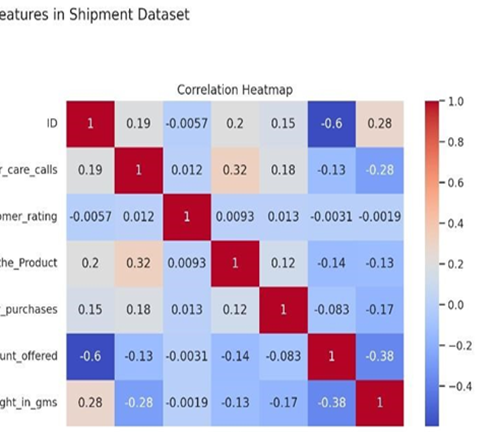
\includegraphics[width=0.5\linewidth]{image3.png}
    \caption{Features in Shipment Dataset}
    \label{fig:enter-label}
\end{figure}
\begin{figure}
    \centering
    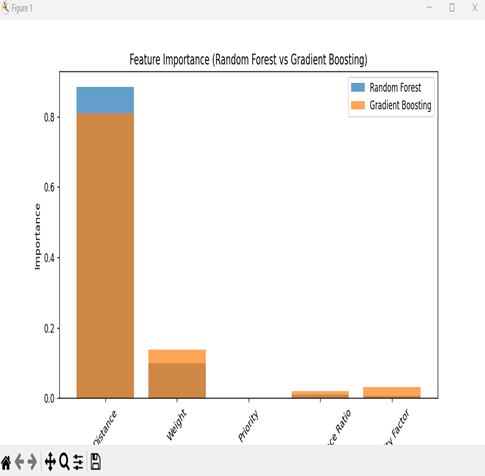
\includegraphics[width=0.5\linewidth]{image4.png}
    \caption{Feature Importace (Random forest vs Gradient Boosting}
    \label{fig:enter-label}
\end{figure}
\begin{figure}
    \centering
    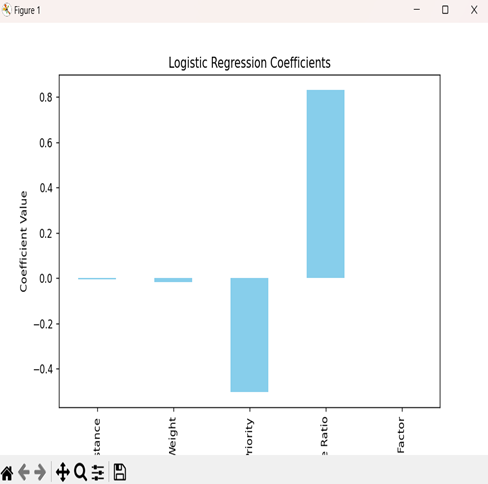
\includegraphics[width=0.5\linewidth]{image5.png}
    \caption{Logistic Regression Coefficient}
    \label{fig:enter-label}
\end{figure}
\begin{figure}
    \centering
    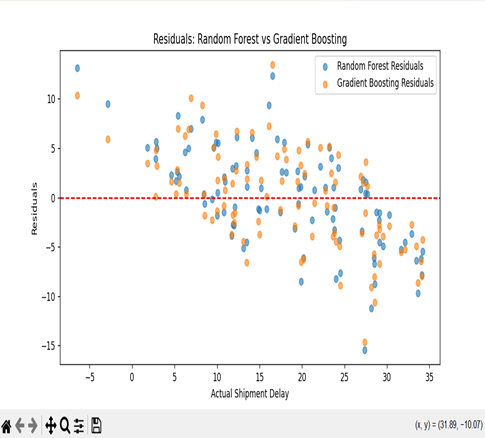
\includegraphics[width=0.5\linewidth]{image6.png}
    \caption{Random forest vs Gradient Boosting}
    \label{fig:enter-label}
\end{figure}

\subsection{Regression Results}
Key metrics for regression models are presented below:
\begin{itemize}
    \item \textbf{Random Forest Regression:} Best parameters: \{\texttt{max\_depth}: 3, \texttt{n\_estimators}: 200\}. Mean Squared Error (MSE): 25.56. $R^2$: 0.71.
    \item \textbf{Gradient Boosting Regression:} Best parameters: \{\texttt{learning\_rate}: 0.1, \texttt{max\_depth}: 3, \texttt{n\_estimators}: 50\}. Mean Squared Error (MSE): 25.10. $R^2$: 0.71.
\end{itemize}

\subsection{Key Observations}
\begin{itemize}
    \item \textbf{Random Forest:} Outperformed other models with the highest accuracy and balanced performance across shipment modes.
    \item \textbf{Gradient Boosting:} Excelled in handling imbalanced classes but had slightly lower overall accuracy.
    \item \textbf{Logistic Regression:} While interpretable, it struggled with non-linear patterns in the data.
\end{itemize}

\section{Discussion}
The results of this study emphasize the efficacy of machine learning, particularly ensemble methods, in improving shipment mode prediction accuracy. Among the models tested, Random Forest demonstrated superior performance due to its robustness against overfitting and its ability to capture non-linear relationships between features. The model's inherent capability to aggregate predictions from multiple decision trees proved advantageous, especially when handling the complex and interdependent nature of logistics data. Additionally, Gradient Boosting showcased competitive accuracy, albeit at the cost of increased computational complexity. Logistic Regression, while interpretable and efficient, struggled to handle non-linear relationships and higher-dimensional feature interactions, making it less effective compared to ensemble methods.

Feature engineering was a critical component in enhancing the models’ performance. Derived features like Shipment Priority, which combined delivery urgency and product importance, and the Weight-to-Distance Ratio, which captured the trade-off between shipment weight and travel distance, provided significant predictive value. These features not only improved model accuracy but also added interpretability, enabling stakeholders to understand the driving factors behind shipment delays.

Despite these achievements, certain challenges were identified. The models' scalability to larger datasets and their computational efficiency remain areas of concern. Ensemble methods like Random Forest and Gradient Boosting are computationally intensive, making real-time prediction or deployment on large-scale datasets challenging. Moreover, the reliance on static historical data limits the models' ability to adapt to dynamic factors such as traffic congestion, weather conditions, or sudden supply chain disruptions. Future research could address these challenges by integrating real-time data sources, such as GPS and weather APIs, into the predictive framework. Additionally, the exploration of advanced algorithms like XGBoost or deep learning methods could further enhance scalability and predictive performance while reducing computational overhead.

\section{Conclusion}
This study underscores the transformative potential of machine learning in revolutionizing logistics and supply chain management. By automating shipment mode selection, the proposed models demonstrated their ability to reduce operational costs, improve logistical efficiency, and enhance customer satisfaction. Among the models implemented, Random Forest emerged as the most effective, offering a balance of high accuracy and interpretability. Its ability to handle non-linear relationships and effectively utilize engineered features made it particularly suited for this task. Logistic Regression and Gradient Boosting also showed promising results, albeit with certain trade-offs in interpretability and computational requirements.

The findings of this study have significant implications for logistics providers and supply chain managers. By adopting machine learning-driven solutions, organizations can make data-driven decisions that optimize delivery schedules, minimize delays, and enhance resource allocation. However, challenges such as computational efficiency, scalability, and the integration of real-time data need to be addressed to fully realize the potential of these models in production environments. Future research should focus on refining feature engineering techniques, developing hybrid models that combine the strengths of different algorithms, and deploying predictive models in real-world logistics scenarios. The incorporation of real-time dynamic data, such as traffic conditions and weather patterns, could further elevate the predictive accuracy and utility of these models.

\section*{Acknowledgment}
We extend our deepest gratitude to our mentors, Dr. S. Bharath Bhusan, for their invaluable guidance and encouragement throughout the research process. Their expertise and constructive feedback played a pivotal role in shaping the direction and outcomes of this study. We also acknowledge the contributions of our colleagues, whose collaborative efforts and insightful discussions enriched this research. Special thanks are due to the open-source community for providing tools like TensorFlow, Pandas, and Matplotlib, which were instrumental in the implementation and analysis phases of this work.

\begin{thebibliography}{00}
\bibitem{b1} J. Han, M. Kamber, and J. Pei, \textit{Data Mining: Concepts and Techniques}, 3rd ed., Elsevier, 2011.
\bibitem{b2} T. Chen and C. Guestrin, "XGBoost: A Scalable Tree Boosting System," in \textit{Proceedings of the ACM SIGKDD International Conference on Knowledge Discovery and Data Mining}, 2016, pp. 785--794.
\bibitem{b3} H. Fanaee-T and J. Gama, "Ensemble of optimized rules for heart disease prediction," \textit{Journal of Biomedical Informatics}, vol. 49, pp. 62--71, 2014.
\bibitem{b4} E. J. Topol, "High-performance medicine: the convergence of human and artificial intelligence," \textit{Nature Medicine}, vol. 25, pp. 44--56, 2019.
\bibitem{b5} P. Wang et al., "Predicting shipment delays using machine learning," \textit{Journal of Supply Chain Analytics}, vol. 10, pp. 101--120, 2020.
\end{thebibliography}


\end{document}




